        %%******************************************%%
        %%                                          %%
        %%        Modello di tesi di laurea         %%
        %%            di Andrea Giraldin            %%
        %%                                          %%
        %%             2 novembre 2012              %%
        %%                                          %%
        %%******************************************%%


% I seguenti commenti speciali impostano:
% 1.
% 2. PDFLaTeX come motore di composizione;
% 3. tesi.tex come documento principale;
% 4. il controllo ortografico italiano per l'editor.

% !TEX encoding = UTF-8
% !TEX TS-program = pdflatex
% !TEX root = tesi.tex
% !TEX spellcheck = it-IT

\documentclass[10pt,                    % corpo del font principale
               a4paper,                 % carta A4
               twoside,                 % impagina per fronte-retro
               openright,               % inizio capitoli a destra
               english,
               italian,
               ]{book}

%**************************************************************
% Importazione package
%**************************************************************

%\usepackage{amsmath,amssymb,amsthm}    % matematica

\usepackage[T1]{fontenc}                % codifica dei font:
                                        % NOTA BENE! richiede una distribuzione *completa* di LaTeX

\usepackage{lmodern}                    % font expansion error

\usepackage[utf8]{inputenc}             % codifica di input; anche [latin1] va bene
                                        % NOTA BENE! va accordata con le preferenze dell'editor

\usepackage[english, italian]{babel}    % per scrivere in italiano e in inglese;
                                        % l'ultima lingua (l'italiano) risulta predefinita

\usepackage{bookmark}                   % segnalibri

\usepackage{caption}                    % didascalie

\usepackage{chngpage,calc}              % centra il frontespizio

\usepackage{csquotes}                   % gestisce automaticamente i caratteri (")

\usepackage{emptypage}                  % pagine vuote senza testatina e piede di pagina

\usepackage{epigraph}			% per epigrafi

\usepackage{eurosym}                    % simbolo dell'euro

%\usepackage{indentfirst}               % rientra il primo paragrafo di ogni sezione

\usepackage{graphicx}                   % immagini

\usepackage{hyperref}                   % collegamenti ipertestuali

\usepackage[binding=5mm]{layaureo}      % margini ottimizzati per l'A4; rilegatura di 5 mm

\usepackage{listings}                   % codici

\usepackage{microtype}                  % microtipografia

\usepackage{mparhack,fixltx2e,relsize}  % finezze tipografiche

\usepackage{nameref}                    % visualizza nome dei riferimenti

\usepackage[font=small]{quoting}        % citazioni

\usepackage{subfig}                     % sottofigure, sottotabelle

\usepackage[italian]{varioref}          % riferimenti completi della pagina

% \usepackage[dvipsnames]{xcolor}         % colori

\usepackage{booktabs}                   % tabelle
\usepackage{tabularx}                   % tabelle di larghezza prefissata
\usepackage{longtable}                  % tabelle su più pagine
\usepackage{ltxtable}                   % tabelle su più pagine e adattabili in larghezza

\usepackage[toc, acronym]{glossaries}   % glossario
                                        % per includerlo nel documento bisogna:
                                        % 1. compilare una prima volta tesi.tex;
                                        % 2. eseguire: makeindex -s tesi.ist -t tesi.glg -o tesi.gls tesi.glo
                                        % 3. eseguire: makeindex -s tesi.ist -t tesi.alg -o tesi.acr tesi.acn
                                        % 4. compilare due volte tesi.tex.

\usepackage[backend=biber,style=verbose-ibid,hyperref,backref]{biblatex}
                                        % eccellente pacchetto per la bibliografia;
                                        % produce uno stile di citazione autore-anno;
                                        % lo stile "numeric-comp" produce riferimenti numerici
                                        % per includerlo nel documento bisogna:
                                        % 1. compilare una prima volta tesi.tex;
                                        % 2. eseguire: biber tesi
                                        % 3. compilare ancora tesi.tex.

\usepackage{float}                      % [H]


% -- DA SWEG
\usepackage{enumitem}
\usepackage{totpages}
\usepackage{tabularx, array}
\usepackage{dcolumn}
\usepackage{epstopdf}
\usepackage{fancyhdr}
% \usepackage{calc}
\usepackage{datatool}
\usepackage[bottom]{footmisc}
\usepackage{textcomp}
\usepackage{titlesec}
\usepackage{rotating}
\usepackage{multirow}
\usepackage{placeins}
\usepackage{color}
\usepackage{makecell}
\usepackage{pdflscape}
\usepackage[table,usenames,dvipsnames]{xcolor}

\definecolor{lightgray}{gray}{0.92}
\definecolor{lightblue}{rgb}{0.93,0.95,1.0}
\definecolor{headgray}{gray}{0.88}
\colorlet{beautyblue}{blue!45}

% Ridefinizione dell'env tabularx. Il vecchio è utilizzabile con l'env oldtabularx
\let\oldtabularx\tabularx
\let\endoldtabularx\endtabularx
\renewenvironment{tabularx}{\rowcolors{2}{white}{lightgray}\oldtabularx}{\endoldtabularx}

% Per tabularx con padding, parametro tra [], eg [1.3]
\newenvironment{paddedtablex}[1][1]{%
	\renewcommand*{\arraystretch}{#1}%
	\renewcommand\theadfont{\bfseries}%
	\tabularx%
}{\endtabularx}


% --



%**************************************************************
% file contenente le impostazioni della tesi
%**************************************************************

%**************************************************************
% Frontespizio
%**************************************************************

% Autore
\newcommand{\myName}{Laura Cameran}
\newcommand{\myTitle}{Un plugin Maven per l'automatizzazione della pubblicazione di documentazione software}

% Tipo di tesi
\newcommand{\myDegree}{Tesi di laurea triennale}

% Università
\newcommand{\myUni}{Università degli Studi di Padova}

% Facoltà
\newcommand{\myFaculty}{Corso di Laurea in Informatica}

% Dipartimento
\newcommand{\myDepartment}{Dipartimento di Matematica "Tullio Levi-Civita"}

% Titolo del relatore
\newcommand{\profTitle}{Prof.}

% Relatore
\newcommand{\myProf}{Paolo Baldan}

% Luogo
\newcommand{\myLocation}{Padova}

% Anno accademico
\newcommand{\myAA}{2018-2019}

% Data discussione
\newcommand{\myTime}{Settembre 2019}


%**************************************************************
% Impostazioni di impaginazione
% see: http://wwwcdf.pd.infn.it/AppuntiLinux/a2547.htm
%**************************************************************

\setlength{\parindent}{14pt}   % larghezza rientro della prima riga
\setlength{\parskip}{0pt}   % distanza tra i paragrafi


%**************************************************************
% Impostazioni di biblatex
%**************************************************************
\bibliography{bibliografia} % database di biblatex

\defbibheading{bibliography} {
    \cleardoublepage
    \phantomsection
    \addcontentsline{toc}{chapter}{\bibname}
    \chapter*{\bibname\markboth{\bibname}{\bibname}}
}

\setlength\bibitemsep{1.5\itemsep} % spazio tra entry

\DeclareBibliographyCategory{opere}
\DeclareBibliographyCategory{web}

\addtocategory{opere}{womak:lean-thinking}
\addtocategory{web}{site:agile-manifesto}

\defbibheading{opere}{\section*{Riferimenti bibliografici}}
\defbibheading{web}{\section*{Siti Web consultati}}


%**************************************************************
% Impostazioni di caption
%**************************************************************
\captionsetup{
    tableposition=top,
    figureposition=bottom,
    font=small,
    format=hang,
    labelfont=bf
}

%**************************************************************
% Impostazioni di glossaries
%**************************************************************
% 
%**************************************************************
% Acronimi
%**************************************************************
% \renewcommand{\acronymname}{Acronimi e abbreviazioni}

% \newacronym[description={\glslink{apig}{Application Program Interface}}]
%     {api}{API}{Application Program Interface}

% \newacronym[description={\glslink{umlg}{Unified Modeling Language}}]
%     {uml}{UML}{Unified Modeling Language}

%**************************************************************
% Glossario
%**************************************************************
% \renewcommand{\glossaryname}{Glossario}

\newglossaryentry{apig}
{
    name=\glslink{api}{API},
    text=Application Program Interface,
    sort=api,
    description={in informatica con il termine \emph{Application Programming Interface API} (ing. interfaccia di programmazione di un'applicazione) si indica ogni insieme di procedure disponibili al programmatore, di solito raggruppate a formare un set di strumenti specifici per l'espletamento di un determinato compito all'interno di un certo programma. La finalità è ottenere un'astrazione, di solito tra l'hardware e il programmatore o tra software a basso e quello ad alto livello semplificando così il lavoro di programmazione}
}

\newglossaryentry{umlg}
{
    name=\glslink{uml}{UML},
    text=UML,
    sort=uml,
    description={in ingegneria del software \emph{UML, Unified Modeling Language} (ing. linguaggio di modellazione unificato) è un linguaggio di modellazione e specifica basato sul paradigma object-oriented. L'\emph{UML} svolge un'importantissima funzione di ``lingua franca'' nella comunità della progettazione e programmazione a oggetti. Gran parte della letteratura di settore usa tale linguaggio per descrivere soluzioni analitiche e progettuali in modo sintetico e comprensibile a un vasto pubblico}
}
 % database di termini
% \makeglossaries


%**************************************************************
% Impostazioni di graphicx
%**************************************************************
\graphicspath{{immagini/}} % cartella dove sono riposte le immagini


%**************************************************************
% Impostazioni di hyperref
%**************************************************************
\hypersetup{
    %hyperfootnotes=false,
    %pdfpagelabels,
    %draft,	% = elimina tutti i link (utile per stampe in bianco e nero)
    colorlinks=true,
    linktocpage=true,
    pdfstartpage=1,
    pdfstartview=FitV,
    % decommenta la riga seguente per avere link in nero (per esempio per la stampa in bianco e nero)
    %colorlinks=false, linktocpage=false, pdfborder={0 0 0}, pdfstartpage=1, pdfstartview=FitV,
    breaklinks=true,
    pdfpagemode=UseNone,
    pageanchor=true,
    pdfpagemode=UseOutlines,
    plainpages=false,
    bookmarksnumbered,
    bookmarksopen=true,
    bookmarksopenlevel=1,
    hypertexnames=true,
    pdfhighlight=/O,
    %nesting=true,
    %frenchlinks,
    urlcolor=webbrown,
    linkcolor=RoyalBlue,
    citecolor=webgreen,
    %pagecolor=RoyalBlue,
    %urlcolor=Black, linkcolor=Black, citecolor=Black, %pagecolor=Black,
    pdftitle={\myTitle},
    pdfauthor={\textcopyright\ \myName, \myUni, \myFaculty},
    pdfsubject={},
    pdfkeywords={},
    pdfcreator={pdfLaTeX},
    pdfproducer={LaTeX}
}

%**************************************************************
% Impostazioni di itemize
%**************************************************************
\renewcommand{\labelitemi}{$\ast$}

%\renewcommand{\labelitemi}{$\bullet$}
%\renewcommand{\labelitemii}{$\cdot$}
%\renewcommand{\labelitemiii}{$\diamond$}
%\renewcommand{\labelitemiv}{$\ast$}


%**************************************************************
% Impostazioni di listings
%**************************************************************
\lstset{
    language=[LaTeX]Tex,%C++,
    keywordstyle=\color{RoyalBlue}, %\bfseries,
    basicstyle=\small\ttfamily,
    %identifierstyle=\color{NavyBlue},
    commentstyle=\color{Green}\ttfamily,
    stringstyle=\rmfamily,
    numbers=none, %left,%
    numberstyle=\scriptsize, %\tiny
    stepnumber=5,
    numbersep=8pt,
    showstringspaces=false,
    breaklines=true,
    frameround=ftff,
    frame=single
}


%**************************************************************
% Impostazioni di xcolor
%**************************************************************
\definecolor{webgreen}{rgb}{0,.5,0}
\definecolor{webbrown}{rgb}{.6,0,0}


%**************************************************************
% Altro
%**************************************************************

\newcommand{\omissis}{[\dots\negthinspace]} % produce [...]

% eccezioni all'algoritmo di sillabazione
\hyphenation
{
    ma-cro-istru-zio-ne
    gi-ral-din
}

\newcommand{\sectionname}{sezione}
\addto\captionsitalian{\renewcommand{\figurename}{Figura}
                       \renewcommand{\tablename}{Tabella}}

\newcommand{\glsfirstoccur}{\ap{{[g]}}}

\newcommand{\intro}[1]{\emph{\textsf{#1}}}

%**************************************************************
% Environment per ``rischi''
%**************************************************************
\newcounter{riskcounter}                % define a counter
\setcounter{riskcounter}{0}             % set the counter to some initial value

%%%% Parameters
% #1: Title
\newenvironment{risk}[1]{
    \refstepcounter{riskcounter}        % increment counter
    \par \noindent                      % start new paragraph
    \textbf{\arabic{riskcounter}. #1}   % display the title before the
                                        % content of the environment is displayed
}{
    \par\medskip
}

\newcommand{\riskname}{Rischio}

\newcommand{\riskdescription}[1]{\textbf{\\Descrizione:} #1.}

\newcommand{\risksolution}[1]{\textbf{\\Soluzione:} #1.}

%**************************************************************
% Environment per ``use case''
%**************************************************************
\newcounter{usecasecounter}             % define a counter
\setcounter{usecasecounter}{0}          % set the counter to some initial value

%%%% Parameters
% #1: ID
% #2: Nome
\newenvironment{usecase}[2]{
    \renewcommand{\theusecasecounter}{\usecasename #1}  % this is where the display of
                                                        % the counter is overwritten/modified
    \refstepcounter{usecasecounter}             % increment counter
    \vspace{10pt}
    \par \noindent                              % start new paragraph
    {\large \textbf{\usecasename #1: #2}}       % display the title before the
                                                % content of the environment is displayed
    \medskip
}{
    \medskip
}

\newcommand{\usecasename}{UC}

\newcommand{\usecaseactors}[1]{\textbf{\\Attori Principali:} #1. \vspace{4pt}}
\newcommand{\usecasepre}[1]{\textbf{\\Precondizioni:} #1. \vspace{4pt}}
\newcommand{\usecasedesc}[1]{\textbf{\\Descrizione:} #1. \vspace{4pt}}
\newcommand{\usecasepost}[1]{\textbf{\\Postcondizioni:} #1. \vspace{4pt}}
\newcommand{\usecasealt}[1]{\textbf{\\Scenario Alternativo:} #1. \vspace{4pt}}

%**************************************************************
% Environment per ``namespace description''
%**************************************************************

\newenvironment{namespacedesc}{
    \vspace{10pt}
    \par \noindent                              % start new paragraph
    \begin{description}
}{
    \end{description}
    \medskip
}

\newcommand{\classdesc}[2]{\item[\textbf{#1:}] #2}





% PRESI DA SWE

\newcommand{\req}[3]{%
#1 & #2 & #3 \\
}

	%COMANDI PER REQ DI FUNZIONALITÀ
	% Generazione automatica dei numeri
	\newcounter{vaF} % valore
	\newcounter{secF}[vaF] % per il secondo livello del requisito
	\newcounter{thF}[secF] % terzo livello

	\newcommand{\ReqF}[3]{\stepcounter{vaF}R\thevaF F#1 & #2 & #3 \\} % Primo livello
	\newcommand{\subReqF}[3]{\stepcounter{secF}R\thevaF.\thesecF F#1 & #2 & #3 \\} % Secondo livello
	\newcommand{\subsubReqF}[3]{\stepcounter{thF}R\thevaF.\thesecF.\thethF F#1 & #2 & #3 \\} % Terzo livello

	% \newcounter{tableCounter} % Per automatizzare conteggio tabelle



	%COMANDI PER REQUISITI DI Qualità
	% Generazione automatica dei numeri
	\newcounter{vaQ} % valore
	\newcounter{secQ}[vaQ]
	\newcounter{thQ}[secQ] % terzo livello

	\newcommand{\ReqQ}[3]{\stepcounter{vaQ}R\thevaQ Q#1 & #2 & #3 \\}
	\newcommand{\subReqQ}[3]{\stepcounter{secQ}R\thevaQ.\thesecQ Q#1 & #2 & #3 \\}
    \newcommand{\subsubReqQ}[3]{\stepcounter{thQ}R\thevaQ.\thesecQ.\thethQ Q#1 & #2 & #3 \\} % Terzo livello



	% COMANDI PER REQ DI VINCOLO
	% Generazione automatica dei numeri

	\newcounter{vaV} % valore
	\newcounter{secV}[vaV]

	\newcommand{\ReqV}[3]{\stepcounter{vaV}R\thevaV V#1 & #2 & #3 \\}
	\newcommand{\subReqV}[3]{\stepcounter{secV}R\thevaV.\thesecV V#1 & #2 & #3 \\}


\newcommand{\bd}[1]{\textbf{#1}}
% \newcommand{\tt}[1]{\texttt{#1}}
\newcommand{\txt}[1]{\texttt{#1}}

% Per i pezzi di codice in Java
\definecolor{dkgreen}{rgb}{0,0.6,0}
\definecolor{gray}{rgb}{0.5,0.5,0.5}
\definecolor{mauve}{rgb}{0.58,0,0.82}

\lstset{frame=tb,
  language=Java,
  aboveskip=3mm,
  belowskip=3mm,
  showstringspaces=false,
  columns=flexible,
  basicstyle={\small\ttfamily},
  numbers=none,
  numberstyle=\tiny\color{gray},
  keywordstyle=\color{blue},
  commentstyle=\color{dkgreen},
  stringstyle=\color{mauve},
  breaklines=true,
  breakatwhitespace=true,
  tabsize=3
}                     % file con le impostazioni personali

\begin{document}
%**************************************************************
% Materiale iniziale
%**************************************************************
\frontmatter
% !TEX encoding = UTF-8
% !TEX TS-program = pdflatex
% !TEX root = ../tesi.tex

%**************************************************************
% Frontespizio 
%**************************************************************
\begin{titlepage}

\begin{center}

\begin{LARGE}
\textbf{\myUni}\\
\end{LARGE}

\vspace{10pt}

\begin{Large}
\textsc{\myDepartment}\\
\end{Large}

\vspace{10pt}

\begin{large}
\textsc{\myFaculty}\\
\end{large}

\vspace{30pt}
\begin{figure}[htbp]
\begin{center}
\includegraphics[height=6cm]{logo-unipd}
\end{center}
\end{figure}
\vspace{25pt} 

\begin{LARGE}
\begin{center}
\textbf{\myTitle}\\
\end{center}
\end{LARGE}

\vspace{10pt} 

\begin{large}
\textsl{\myDegree}\\
\end{large}

\vspace{35pt} 

\begin{large}
\begin{flushleft}
\textit{Relatore}\\ 
\vspace{5pt} 
\profTitle \myProf
\end{flushleft}

\vspace{0pt} 

\begin{flushright}
\textit{Laureanda}\\ 
\vspace{5pt} 
\myName
\end{flushright}
\end{large}

\vspace{32pt}

\line(1, 0){338} \\
\begin{normalsize}
\textsc{Anno Accademico \myAA}
\end{normalsize}

\end{center}
\end{titlepage} 
\input{inizio-fine/colophon}
% !TEX encoding = UTF-8
% !TEX TS-program = pdflatex
% !TEX root = ../tesi.tex

%**************************************************************
% Dedica
%**************************************************************
\cleardoublepage
\phantomsection
\thispagestyle{empty}
\pdfbookmark{Dedica}{Dedica}

\vspace*{3cm}

\begin{center}
    ``I made a discovery today.  I found a computer. \\
    Wait a second, this is cool.  It does what I want it to. \\
    If it makes a mistake, it's because I screwed it up.  Not because it doesn't like me.'' \\ \medskip
--- The Mentor    
\end{center}

\medskip

% \begin{center}
% Dedicato a ...
% \end{center}

% !TEX encoding = UTF-8
% !TEX TS-program = pdflatex
% !TEX root = ../tesi.tex

%**************************************************************
% Sommario
%**************************************************************
\cleardoublepage
\phantomsection
\pdfbookmark{Sommario}{Sommario}
\begingroup
\let\clearpage\relax
\let\cleardoublepage\relax
\let\cleardoublepage\relax

\chapter*{Sommario}

Il documento corrent descrive il lavoro svolto durante il periodo di stage, della durata di trecentoventi ore, dalla laureanda Laura Cameran presso l'azienda Finantix Pro S.r.l.
Gli obiettivi da raggiungere erano molteplici.\\
In primo luogo era richiesto lo sviluppo di ...
In secondo luogo era richiesta l'implementazione di un ... 
Tale framework permette di registrare gli eventi di un controllore programmabile, quali segnali applicati 
Terzo ed ultimo obbiettivo era l'integrazione ...

%\vfill
%
%\selectlanguage{english}
%\pdfbookmark{Abstract}{Abstract}
%\chapter*{Abstract}
%
%\selectlanguage{italian}

\endgroup			

\vfill


% % !TEX encoding = UTF-8
% !TEX TS-program = pdflatex
% !TEX root = ../tesi.tex

%**************************************************************
% Ringraziamenti
%**************************************************************
\cleardoublepage
\phantomsection
\pdfbookmark{Ringraziamenti}{ringraziamenti}

%\begin{flushright}{
%	\slshape    
%	``Life is really simple, but we insist on making it complicated''} \\ 
%	\medskip
%    --- Confucius
%\end{flushright}


\bigskip

\begingroup
\let\clearpage\relax
\let\cleardoublepage\relax
\let\cleardoublepage\relax

\chapter*{Ringraziamenti}

\noindent \textit{Innanzitutto, vorrei esprimere la mia gratitudine al Prof. NomeDelProfessore, relatore della mia tesi, per l'aiuto e il sostegno fornitomi durante la stesura del lavoro.}\\

\noindent \textit{Desidero ringraziare con affetto i miei genitori per il sostegno, il grande aiuto e per essermi stati vicini in ogni momento durante gli anni di studio.}\\

\noindent \textit{Ho desiderio di ringraziare poi i miei amici per tutti i bellissimi anni passati insieme e le mille avventure vissute.}\\
\bigskip

\noindent\textit{\myLocation, \myTime}
\hfill \myName

\endgroup


\input{inizio-fine/indici}
\cleardoublepage

%**************************************************************
% Materiale principale
%**************************************************************
\mainmatter
% !TEX encoding = UTF-8
% !TEX TS-program = pdflatex
% !TEX root = ../tesi.tex

%**************************************************************
\chapter{Introduzione}
\label{cap:introduzione}
%**************************************************************

% Introduzione al contesto applicativo.\\

% \noindent Esempio di utilizzo di un termine nel glossario \\
% \gls{api}. \\

% \noindent Esempio di citazione in linea \\
% \cite{site:agile-manifesto}. \\

% \noindent Esempio di citazione nel pie' di pagina \\
% citazione\footcite{womak:lean-thinking} \\

%**************************************************************
\section{Il progetto}   \label{secProgetto}
%Descrizione dell'azienda.
Finantix è un'azienda di informatica che vende un prodotto software principale.
Questo prodotto, per la realizzazione di applicazioni finanziarie, è suddiviso in moduli.
Ognuno di questi moduli prevede una propria documentazione delle API Java (un archivio zip contente documentazione in formato JavaDoc) e la documentazione della API RESTful (un archivio zip contenente documentazione in formato Open API).
Questa documentazione viene manualmente caricata sulla piattaforma Confluence, ove cui è consultata dagli sviluppatori dell'azienda.

%Introduzione all'idea dello stage.
Il plugin Maven nasce dalla necessità di automatizzare la pubblicazione di questa documentazione sulla piattaforma, in modo da semplificare e velocizzare notevolmente questo processo.
Infatti, una volta configurato correttamente il plugin in tutti i progetti relativi ai moduli software, il caricamento della documentazione avviene direttamente durante la build del progetto, senza richiedere ulteriore intervento umano.

    
    Il progetto ha avuto inizio il 10 giugno 2019 ed ha terminato il 2 agosto 2019, per un totale di 320 ore.

    Durante queste 8 settimane, i prodotti attesi erano:
    \begin{enumerate}
        \item \bd{plug-in Maven}: progetto Java il cui risultato è il plugin sopra descritto;
        \item \bd{manuale dell’utilizzatore}: documentazione del plugin Maven che illustra come attivarlo e configurarlo al fine di pubblicare la documentazione generata durante il processo di build sul sistema documentale dell’azienda;
        \item \bd{manuale del programmatore}: descrizione tecnica del plugin Maven, vale a dire, le classi principali dell’implementazione con le relative responsabilità ed il relativo funzionamento.
    \end{enumerate}

    Per raggiungere questo scopo, sono stati fissati alcuni fondamentali obiettivi:
    \begin{itemize}
        \item studiare in maniera autonoma lo strumento Maven per poterne capire appieno l'utilità ed il funzionamento;
        \item comprendere come realizzazione un plugin Maven, oggetto centrale del progetto;
        \item comprendere il paradigma RESTful, per poter trasmettere dati al server documentale;
        \item implementare il plugin Maven, una volta raggiunte le competenze sufficienti;
        \item realizzare la documentazione utente, ovvero il manuale dell'utilizzatore sopra citato, per semplificare la comprensione dell'utilizzo del plugin all'utente finale. Non è strettamente necessario all'adempimento del plugin Maven, ma auspicabile;
        \item realizzare la documentazione dello sviluppatore, ovvero il manuale del programmatore sopra citato, per aiutare il programmatore nella cognizione del codice. Anch'esso, come il punto precedente, non è necessario ma auspicabile;
        \item impiegare la tecnologia Jenkins che è usata per ogni progetto per la continuos integration. Per questo motivo, è possibile farne un minimo utilizzo, ma non è strettamente richiesto.
    \end{itemize}
    
    Tutti gli obiettivi possono essere tracciati da un codice univoco che li identifica. 
    Ognuno di essi ha inoltre una determinata priorità scelta in base all'importanza e necessità di raggiungerli.
    La tabella \ref{obiettiviProgetto} li riassume.
    \begin{table}[H]
		\begin{paddedtablex}[1.7]{\textwidth}{cXc}
			\rowcolor{beautyblue}\textbf{Codice} & \textbf{Descrizione} & \textbf{Priorità} \\
			\toprule
			
            O01 & Acquisizione competenze su Maven & Obbligatorio \\
            O02 & Acquisizione competenze sull’implementazione di plugin Maven & Obbligatorio \\
            O03 & Familiarità con il paradigma RESTFul & Obbligatorio \\
            O04 & Implementazione di un plugin Maven & Obbligatorio \\
            D01 & Documentazione per l’utilizzatore & Desiderabile \\
            D02 & Documentazione per il programmatore & Desiderabile \\
            F01 & Utilizzo di base di Jenkins & Facoltativo \\

			\bottomrule
		\end{paddedtablex}
        \caption{Obiettivi del progetto}
        \label{obiettiviProgetto}
	\end{table}
  
% TODO ampliare 
% Nel piano di lavoro è presente un prospetto che settimana per settimana indica quali attività vengono svolte. L'hai riportato nella tesi? Se l'hai riportato, hai indicato le modifiche all'ordine con cui sono state svolte le attività?




%**************************************************************
\section{Principali problematiche}
Durante il corso dello stage non sono stati riscontrati rilevanti problemi che hanno particolarmente influito sull'attività.
Nonostante ciò, un problema non banale che è stato affrontato riguarda la documentazione di Maven.
Molte pagine relative alla documentazione di plugin Maven infatti, risultano obsolete perché poco aggiornate.
Per far fronte a questo problema, un confronto diretto e costante con gli sviluppatori senior del team DevOps, esperti della tecnologia, è stato il metodo di risoluzione determinante.


%**************************************************************
\section{Strumenti utilizzati}
Gli strumenti adottati per la creazione del plugin Maven sono molteplici.
Alcune di questi sono abitualmente adoperati da tutti gli sviluppatori dell'azienda, motivo per cui sono stati utilizzati anche per questo progetto, mentre altri sono stati liberamente scelti dalla candidata.
Tra essi, scelti selezionati per i vari motivi sotto elencati, troviamo:
\begin{itemize}
    \item \textbf{GitKraken}: client di Git che presenta un'interfaccia grafica molto intuitiva e interattiva, oltre che semplice da usare;
    % \item \textbf{JUnit}: framework per i test d'unità che si integra facilmente con Eclipse e Maven
    \item \textbf{Visual Studio Code}: editor di codice che supporta molti linguaggi, tra cui JSON e HTML \cite{site:visual-studio-code};
    \item \bd{SequenceDiagram.org}: strumento online che permette la creazione di diagrammi di sequenza in modo semplice e veloce grazie ad una sintassi propria;
    \item \bd{ObjectAid UML Explorer}: strumento d'integrazione a Eclipse che permette la creazione automatica di diagrammi delle classi a partire dal codice Java;
    \item \bd{Meecrowave}: framework consigliato dall'azienda (ma non imposto) che permette la creazione di server velocemente \cite{site:meecrowave}.
\end{itemize}

    \subsection{Maven} \label{mavenSection} % TODO rileggere
        
    Maven \cite{site:maven-introduzione} è un software per la gestione di progetti, basato sul concetto di un ``project object model'' (POM), che gli permette di gestire la build, il report e la documentazione di un progetto Java da un unico pezzo di informazione centrale.

    % -------- LIFE CYCLE
    Maven è basato sul concetto di un ciclo di vita della build \cite{site:maven-lifecycle}.
    Ciò significa che il processo per la build e la distribuzione di un particolare artefatto (progetto) è chiaramente definito. 
    Per la persona che realizza un progetto, ciò significa che è solamente necessario imparare un piccolo set di comandi per eseguire la build di un progetto e il POM assicurerà l'ottenimento dei risultati desiderati.
    Ci sono diversi cicli di vita possibili ed ogni ciclo di vita è suddiviso in fasi ben determinate.
    Per esempio, una fase di particolare rilevanza per il progetto del plugin Maven è la fase di \emph{package}, che si occupa di prendere il codice compilato e impacchettarlo nel suo formato distribuibile, come per esempio un JAR. 

    % ------------------

    Ciò che è possibile gestire con questo POM è, per esempio, la lista di dipendeze e i report dei test d'unità, incluso il coverage.
    Il suo aspetto è quello di un file XML che contiene le informazioni riguardanti il progetto e i dettagli della configurazione, usati da Maven per fare la build dei progetti.

    % -------- PLUGIN
    \subsubsection{Cos'è un plugin Maven}

    Un plugin Maven è un programma non autonomo che interagisce con Maven per ampliarne o estenderne le funzionalità originarie \cite{site:maven-plugin}.

    Essendo il progetto incentrato sulla realizzazione di un plugin Maven, esso deve avere un \emph{goal}.
    Un \emph{goal} rappresenta un compito specifico (è più fine di una fase) che contribuisce alla gestione del progetto.
    Può essere legato a nessuna, una o più fasi della build.
    Un \emph{goal} non legato ad alcuna fase può essere eseguito al di fuori del ciclo di vita, tramite un'invocazione diretta.


    Quando viene eseguito un goal, Maven cerca il file ``pom.xml'' (il POM) nella cartella corrente, lo legge, ottiene le informazioni della configurazione e dopo di che esegue il goal.

    Alcune di queste informazioni di configurazione che possono essere specificate nel POM sono dipendeze, i plugin o goal che possono essere eseguiti, la versione del progetto, la descrizione del progetto, ecc \cite{site:maven-pom}.
    A continuazione, viene riportato un esempio.

    % \newpage

    \lstset{frame=tb,
    language=XML,
    aboveskip=3mm,
    belowskip=3mm,
    showstringspaces=false,
    columns=flexible,
    basicstyle={\small\ttfamily},
    numbers=none,
    numberstyle=\tiny\color{gray},
    keywordstyle=\color{black},
    commentstyle=\color{black},
    stringstyle=\color{black},
    breaklines=true,
    breakatwhitespace=true,
    tabsize=3
    }
    \begin{lstlisting} 
    <project>
        <modelVersion>4.0.0</modelVersion>
        <parent>
            <groupId>com.thedigitalstack.maven.plugins</groupId>
            <artifactId>maven-plugins</artifactId>
            <version>1.3.1-SNAPSHOT</version>
        </parent>
        <artifactId>tds-docs-publisher-plugin</artifactId>
        <packaging>maven-plugin</packaging>

        <name>Maven Docs Publisher Plugin</name>
        <description>Maven plug-in to publish generated documentation to 
        Confluence so that official documentation is always up to date with the 
        binary release and easily accessible to authorized users.</description>
        ...
    </project>  
    \end{lstlisting}
    
    % \begin{figure}[H]
    %     \centering
    %     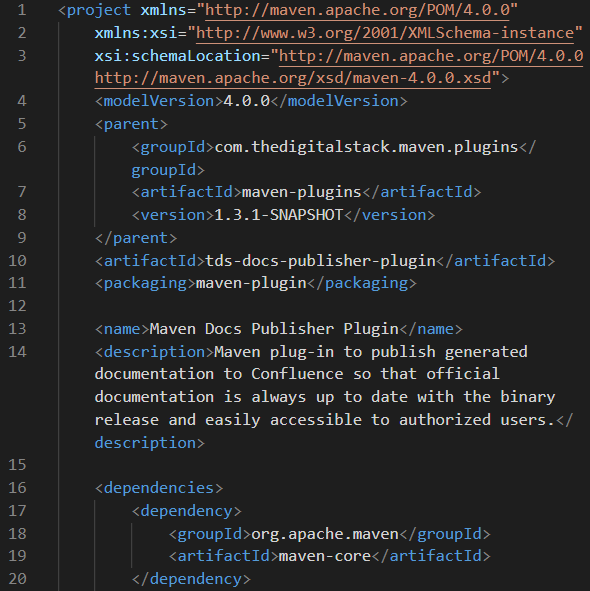
\includegraphics[width=\textwidth]{immagini/screenPOM2.png}\\
    %     \caption{Screenshot di un esempio di POM}
    %     \label{screenPOM}
    % \end{figure}

    % ------------------

    \subsection{Confluence}
    Confluence è un software di collaborazione sviluppato dalla compagnia australiana Atlassian \cite{site:confluence}.
    Esso è il principale sistema documentale dell'azienda, infatti viene usato da ogni dipendente per la consultazione di vario materiale: dalle norme aziendali, alla documentazione del codice.
    Ciò che è più importante, motivo per cui viene utilizzato, è il fatto che permette di raggruppare pagine correlate in uno spazio dedicato accessibile a tutti o a gruppi ristretti di persone.
    
    Recentemente è stato introdotto a Confluence un plugin di terze parti, chiamato \emph{Docs}. 
    Per poter comprendere appieno il progetto del plugin Maven, è prima necessario fare luce su questo plugin.

    \subsubsection{Il plugin Docs} \label{pluginDocs}

    \begin{figure}[H]
        \centering
        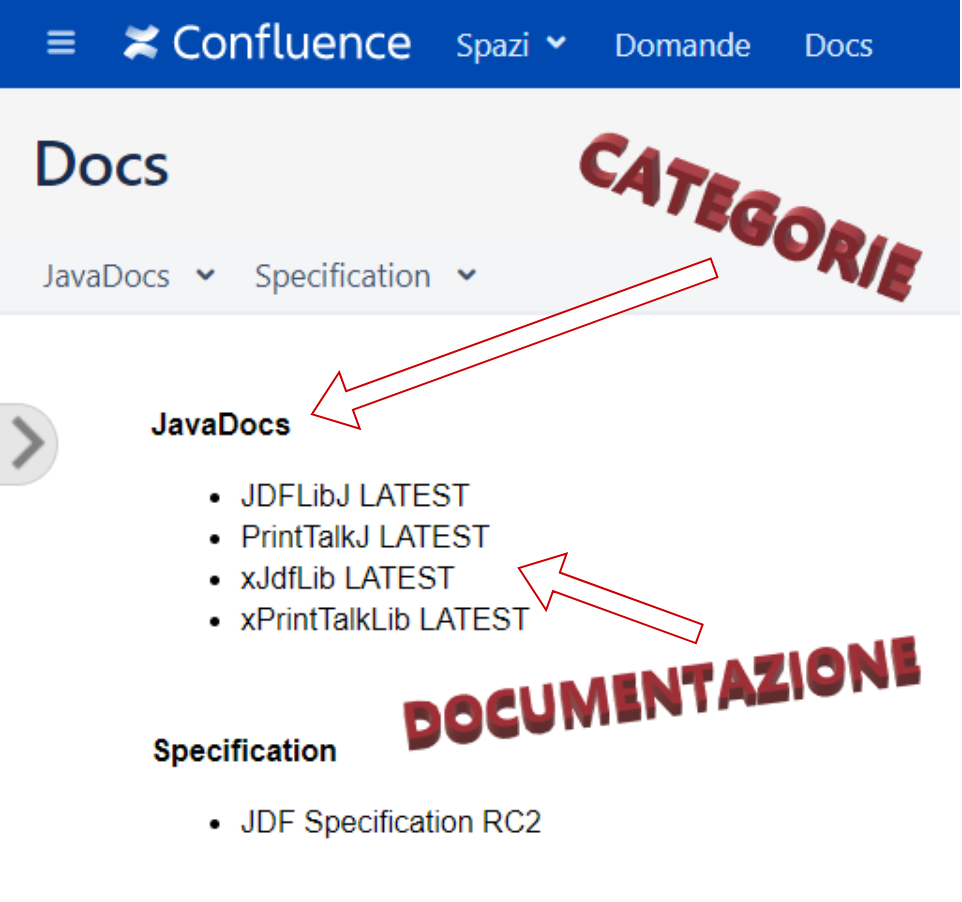
\includegraphics[width=0.56\textwidth]{immagini/docs-conf.png}\\
        \caption{Screenshot di un esempio di Docs Plug-in}
        \label{screenDocs}
    \end{figure}

    Come è possibile vedere dall'immagine \ref{screenDocs}, \emph{Docs} è suddiviso in categorie (in questo caso ``JavaDocs'' e ``Spacification'').
    Le categorie presentano un nome, consentono di raggruppare la documentazione e possono essere collegate agli spazi Confluence esistenti, in modo da permettere la visione di questa documentazione solo a determinate persone.
    Ogni categoria quindi contiene al suo interno delle pagine web (chiamate anche \emph{doc}) che includono la documentazione in formato HTML \cite{site:docs-plugin} (come per esempio ``JDF Specification RC2'' per la categoria ``Specification'').

    % \clearpage

    \subsection{Riepilogo degli strumenti}

    In seguito viene riportata una tabella (\ref{tabellaStrumenti}) che riassume tutti gli strumenti utilizzati e a quale scopo.

        \begin{table}[H]
            {\def\arraystretch{1.5}
            \begin{tabularx}{\textwidth}{cX}
                \rowcolor{beautyblue}
                \textbf{Strumento} &
                \textbf{Scopo} \\ \hline
                Java & Linguaggio di programmazione \\
                Eclipse & Ambiente di sviluppo \\
                Maven & Build automation per la gestione di progetti \\
                Confluence & Pubblicazione, creazione e consultazione di documentazione \\
                Jira & Issue tracking system \\
                Jenkins & Continuous integration \\
                SonarQube & Analisi statica del codice \\
                Bitbucket e GitKraken & Controllo di versione \\
                JUnit & Test di unità \\
                Visual Studio Code & Editor di codice \\
                SequenceDiagram.org & Creazione dei diagrammi di sequenza \\
                ObjectAid UML Explorer & Creazione dei diagrammi delle classi \\
                Meecrowave & Creazione di server \\
            \end{tabularx}} \\
        \caption{Tabella di tecnologie utilizzate durante il progetto e loro scopo.}
        \label{tabellaStrumenti}
        \end{table}


%**************************************************************
\section{Il prodotto ottenuto}
Il plugin Maven riesce a realizzare il caricamento di documentazione grazie ad un plugin di terze parti su Confluence, chiamato \emph{Docs}, descritto nella sezione \S\ref{pluginDocs}.

Ciò che fa il plugin Maven è caricare su \emph{Docs} in maniera automatica la documentazione nella corretta categoria, realizzando un nuovo \emph{doc} o aggiornandone uno esistente.

Nel caso in cui l'utilizzatore del plugin Maven fornisca un titolo per la pagina \emph{doc} che non è presente nel \emph{Docs}, verrà creata una nuova pagina, altrimenti il \emph{doc} già esistente con quel nome verrà aggiornato con la documentazione data.

%**************************************************************
\section{Organizzazione del testo}

\begin{description}
    \item[{\hyperref[cap:analisi-requisiti]{Il secondo capitolo}}] comprende l'analisi dettagliata del prodotto, elencandone successivamente i relativi requisiti individuati.

    \item[{\hyperref[cap:progettazione]{Il terzo capitolo}}] spiega la progettazione e la realizzazione del software, descrivendo le tecnologie utilizzate e l'organizzione del codice tramite diagrammi.

    \item[{\hyperref[cap:testing]{Il quarto capitolo}}] approfondisce come è stata effettuata l'attività di verifica e validazione, soffermandosi in particolare sull'analisi statica del codice e il testing.

    \item[{\hyperref[cap:conclusioni]{Il quinto capitolo}}] corrisponde al capitolo conclusivo. Esso riassume il risultato finale ottenuto e attua una valutazine critica del prodotto.

\end{description}

Riguardo la stesura del testo, relativamente al documento sono state adottate le seguenti convenzioni:
\begin{itemize}
	% \item gli acronimi, le abbreviazioni e i termini ambigui o di uso non comune menzionati vengono definiti nel glossario, situato alla fine del presente documento;
	% \item per la prima occorrenza dei termini riportati nel glossario viene utilizzata la seguente nomenclatura: \emph{parola}\glsfirstoccur;
	\item i termini in lingua straniera o facenti parti del gergo tecnico sono evidenziati con il carattere \emph{corsivo};
	\item per tutti i concetti che possono essere riassunti, viene fornita una tabella o un elenco puntato;
	\item citazioni e riferimenti provenienti da siti o libri vengono accompagnati dal loro numero identificativo tra parentesi quadre, ad esempio \cite{site:junit-annotation}.
\end{itemize}             % Introduzione
% !TEX encoding = UTF-8
% !TEX TS-program = pdflatex
% !TEX root = ../tesi.tex

%**************************************************************
% \chapter{Processi e metodologie}
% \label{cap:processi-metodologie}
%**************************************************************

% \intro{Brevissima introduzione al capitolo}\\

%**************************************************************
% \section{Processo sviluppo prodotto}             % Processi
% !TEX encoding = UTF-8
% !TEX TS-program = pdflatex
% !TEX root = ../tesi.tex

%**************************************************************
% \chapter{Descrizione dello stage}
% \label{cap:descrizione-stage}
%**************************************************************

% \intro{Breve introduzione al capitolo}\\

%**************************************************************
% \section{Introduzione al progetto}

%**************************************************************
% \section{Analisi preventiva dei rischi}

% Durante la fase di analisi iniziale sono stati individuati alcuni possibili rischi a cui si potrà andare incontro.
% Si è quindi proceduto a elaborare delle possibili soluzioni per far fronte a tali rischi.\\

% \begin{risk}{Performance del simulatore hardware}
%     \riskdescription{le performance del simulatore hardware e la comunicazione con questo potrebbero risultare lenti o non abbastanza buoni da causare il fallimento dei test}
%     \risksolution{coinvolgimento del responsabile a capo del progetto relativo il simulatore hardware}
%     \label{risk:hardware-simulator} 
% \end{risk}

%**************************************************************
% \section{Requisiti e obiettivi}


%**************************************************************
% \section{Pianificazione}             % Kick-Off
% !TEX encoding = UTF-8
% !TEX TS-program = pdflatex
% !TEX root = ../tesi.tex

%**************************************************************
\chapter{Analisi dei requisiti}
\label{cap:analisi-requisiti}
%**************************************************************

\intro{Tale capitolo ha l’obiettivo di esporre e analizzare i requisiti espliciti e impliciti per la realizzazione del plugin Maven per la pubblicazione di documentazione software.
L'attività di analisi ha funto da base per la fase di progettazione del software, in modo che il prodotto fosse conforme alle richieste dell’azienda.}

% \section{Casi d'uso}

% Per lo studio dei casi di utilizzo del prodotto sono stati creati dei diagrammi.
% I diagrammi dei casi d'uso (in inglese \emph{Use Case Diagram}) sono diagrammi di tipo \gls{uml} dedicati alla descrizione delle funzioni o servizi offerti da un sistema, così come sono percepiti e utilizzati dagli attori che interagiscono col sistema stesso.
% Essendo il progetto finalizzato alla creazione di un tool per l'automazione di un processo, le interazioni da parte dell'utilizzatore devono essere ovviamente ridotte allo stretto necessario. Per questo motivo i diagrammi d'uso risultano semplici e in numero ridotto.

% \begin{figure}[!h]
%     \centering
%     \includegraphics[width=0.9\columnwidth]{usecase/scenario-principale}
%     \caption{Use Case - UC0: Scenario principale}
% \end{figure}

% \begin{usecase}{0}{Scenario principale}
% \usecaseactors{Sviluppatore applicativi}
% \usecasepre{Lo sviluppatore è entrato nel plug-in di simulazione all'interno dell'IDE}
% \usecasedesc{La finestra di simulazione mette a disposizione i comandi per configurare, registrare o eseguire un test}
% \usecasepost{Il sistema è pronto per permettere una nuova interazione}
% \label{uc:scenario-principale}
% \end{usecase}


% \begin{usecase}{1}{Configurazione}
% \usecaseactors{Sviluppatore}
% \usecasepre{Lo sviluppatore sta utilizzando il progetto}
% \usecasedesc{Lo sviluppatore configura come }
% \usecasepost{Il sistema è pronto per l'esecuzione}
% \label{uc:scenario-principale}
% \end{usecase}

\section{Premessa}
Il prodotto realizzato è un plugin Maven e possiede come nome ufficiale: \emph{Maven documentation publisher plug-in}.

L'obiettivo all'inizio dello stage era il semplice caricamento di documentazione archiviata su \emph{Docs}, per questo motivo è stato scelto di creare il goal denominato \emph{publish}.
Successivamente, nel corso dello stage, sono state aggiunte delle nuove funzionalità e un nuovo goal, dato che le tempistiche pianificate erano ottimistiche e hanno permesso sufficiente tempo per ampliare il prodotto.


\section{Descrizione del prodotto} \label{descrizioneProdotto}

Maven documentation publisher plug-in supporta la pubblicazione di documentazione in formato HTML. Ha due goal:
\begin{itemize}
	\item \bd{publish}: che pubblica la documentazione;
	\item \bd{cleanup}: che elimina la documentazione contenente SNAPSHOT nel nome.
\end{itemize}
Il principale è \emph{publish} e si occupa della pubblicazione su  \emph{Docs} Confluence della documentazione del codice di un qualunque progetto Maven su cui è configurato il plugin.
Questo è possibile perché il plugin Docs di Confluence accetta archivi, ovvero file con estensione .zip o .jar.
La documentazione in questo formato può essere per esempio la documentazione Javadoc (documentazione del codice sorgente scritto in linguaggio Java) o Open API (specifica per file di interfaccia leggibili dalle macchine per descrivere servizi web RESTful, conosciuta anche come specifica Swagger \cite{site:specifica-openapi}).
Entrambe Javadoc e Open API sono il tipo di documentazione di maggior interesse per l'azienda da pubblicare su Docs. \\
Ogni archivio caricato contribuisce alla creazione di una pagina \emph{doc} ed ogni \emph{doc} viene identificato univocamente all'interno di una categoria, per questo motivo, il titolo deve essere unico.
Una pagina viene creata se il titolo della documentazione è nuovo, altrimenti la pagina già esistente viene semplicemente aggiornata. \\ 
 
\subsection{Il goal \emph{publish}} \label{goalPublish}
\emph{Maven documentation publisher plug-in} è altamente configurabile, in modo da soddisfare qualunque esigenza dello sviluppatore.
Innanzitutto esso consente all'utente di inserire:
\begin{itemize}
	\item la documentazione;
	\item le proprie credenziali per accedere a Confluence;	
	\item il nome della categoria in cui allocare la documentazione.
\end{itemize}
La documentazione che fornisce l'utente può essere di tre tipi:
\begin{enumerate}
	\item archivio (ZIP o JAR);
	\item cartella (contenente più file HTML);
	\item singolo file (HTML).
\end{enumerate}
Nei casi 2. e 3. il plugin si occupa anche dell'archiviazione per permettere a Docs di mostrare correttamente la documentazione su Confluence. \\
I possibili modi per fornire le credenziali sono molteplici:
\begin{itemize}
	\item username e password vengono date direttamente nei campi della configurazione a loro destinati;
	\item username e password vengono prese dalla sezione server del file ``.m2/settings.xml'' in cui sono salvate criptate. \footnote{A questo scopo, l'utente deve aver prima proceduto con la criptazione delle proprie credenziali come spiegato alla pagina \url{https://maven.apache.org/guides/mini/guide-encryption.html}} 
\end{itemize}
Non è necessario che l'utente provveda ad entrambi, ma almeno uno ci deve sempre essere.
Se ci sono entrambi, il plugin utilizza il prelevamento dal file ``settings.xml''. \\

Il sistema richiede obbligatoriamente che l'utente fornisca le informazioni sopra descritte.
Oltre a questi parametri però, esistono altri parametri per cui il sistema prevede una configurazione di default, ma che possono essere facoltativamente cambiato dall'utente. 

	\subsubsection{Parametri opzionali} \label{parametriOpzionali}
	L'utente può scegliere nome e versione della documentazione.
	Il titolo della pagina \emph{doc} viene costruito dall'unione di nome e versione (ad esempio dati il nome ``Docs Maven Plugin'' e la versione ``2019'', il titolo apparirà come: ``Docs Maven Plugin 2019'').


	% -------------------------

	Nel caso in cui l'utente non fornisca nome o versione, o nessuno dei due, il sistema prevede il seguente comportamento per i due parametri:
	\begin{itemize}
		\item \bd{nome}: preso dal nome del progetto o alternativamente dall'\emph{artifactId} (identificativo di un progetto Maven);
		\item \bd{versione}: preso dalla versione del progetto.
	\end{itemize} 

	Vengono riportati qui di seguito alcuni esempi (in grassetto vengono evidenziati i valori dati dall'utente per la documentazione, i restanti sono altri elementi configurabili nel POM di un generico progetto Maven):
	\begin{enumerate}
		\item \bd{nome documentazione}: Quickstart Doc,
		\bd{versione documentazione}: 2019,
		 nome progetto: Quickstart Vogella project,  
		 versione progetto: 2.1.1-SNAPSHOT,
		 artifactId: quickstart
		\item nome progetto: Quickstart Vogella project, 
		 versione progetto: 2.1.1-SNAPSHOT, 
		  artifactId: quickstart
		\item \bd{versione documentazione}: 2018,
		 versione progetto: 2.1.1-SNAPSHOT, 
		  artifactId: quickstart
	\end{enumerate}

	\begin{figure}[H]
		\centering
		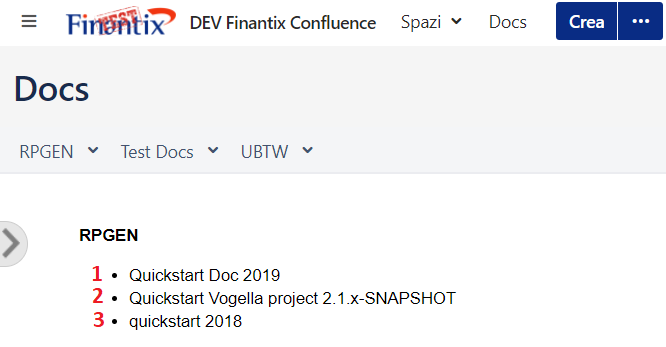
\includegraphics[width=0.88\textwidth]{immagini/DocsExamples.png}\\
		\caption{Esempi di titoli di pagine doc}
		\label{screenDocsNameVersion}
	\end{figure}

	Come è possibile vedere dall'immagine \ref{screenDocsNameVersion}, nel caso 1. vengono dati dall'utente sia nome che versione della documentazione, per questo il titolo viene costruito con questi valori. 
	Nel caso 2. invece non viene fornito nessuno dei due e per questo vengono utilizzati il nome e la versione del progetto. 
	Nel caso 3. viene data solo la versione della documentazione, che infatti viene preferita alla versione del progetto, ma non il nome della documentazione. 
	Poiché nemmeno il nome del progetto è configurato nel POM del progetto, viene scelto di utilizzare l'ultima opzione rimanente: l'artifactId.

	% ---------------------------

	% \newpage

	L'utente può inoltre decidere di impostare:
	\begin{itemize}
		\item lo skip (salto) dell'esecuzione del plugin;
		\item che il plugin non fallisca nel caso in cui accada qualche errore del client;
		\item i tipi di progetto supportati dal plugin e quelli a cui il plugin non deve dare dei warning (messaggi di avvertimento);
		\item che il plugin non fallisca nel caso in cui il percorso all'archivio dato dall'utente come documentazione non esista.
	\end{itemize}

	Per di più, nel caso in cui la documentazione non sia di tipo archivio, bensì il percorso ad una cartella, è possibile dare delle ulteriori istruzioni:
	\begin{itemize}
		\item dove salvare l'archivio creato;
		\item quali tipi di file includere ed escludere dall'archivio.
	\end{itemize}

	Ogni archivio caricato su \emph{Docs} plugin di Confluence deve contenere al suo interno una pagina denominata \emph{main entrance page}, la quale essenzialmente è la prima pagina che viene visualizzata quando si entra in un \emph{doc}.
	Questa è impostata di default nel plugin come ``index.html''.
	Per questo motivo è stato scelto di permettere a \emph{Maven documentation publisher plug-in} di creare questo file qualora mancasse.
	Esso indirizza automaticamente al file principale della documentazione: un file scelto dall'utente tramite l'inserimento del nome in fase di configurazione.

	La figura \ref{errorDocs} mostra Docs nel caso di main entrance page mancante.

	\begin{figure}[H]
		\centering
		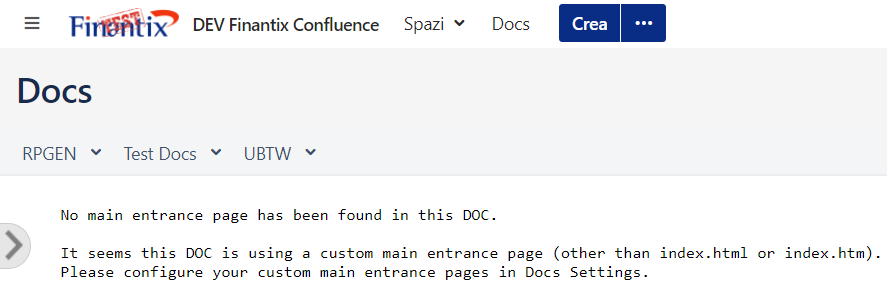
\includegraphics[width=\textwidth]{immagini/indexError.png}\\
		\caption{Esempio di Docs nel caso di file ``index.html'' mancante}
		\label{errorDocs}
	\end{figure}


\subsection{Il goal \emph{cleanup}}
Il secondo goal, \emph{cleanup}, è nato dalla necessità di eliminare la documentazione relativa ad un prodotto che non è stato rilasciato.
Questo tipo di prodotti presentano ``SNAPSHOT'' nella versione e per questo motivo, anche il titolo della pagina \emph{doc} lo contiene.
Si ha quindi qui a che vedere con la pulizia totale dal plugin \emph{Docs} di tutte queste pagine. \\
A questo scopo non è necessario aggiungere nulla alla configurazione del plugin: sono sufficienti le credenziali dell'utente. 

\begin{figure}[H]
	\centering
	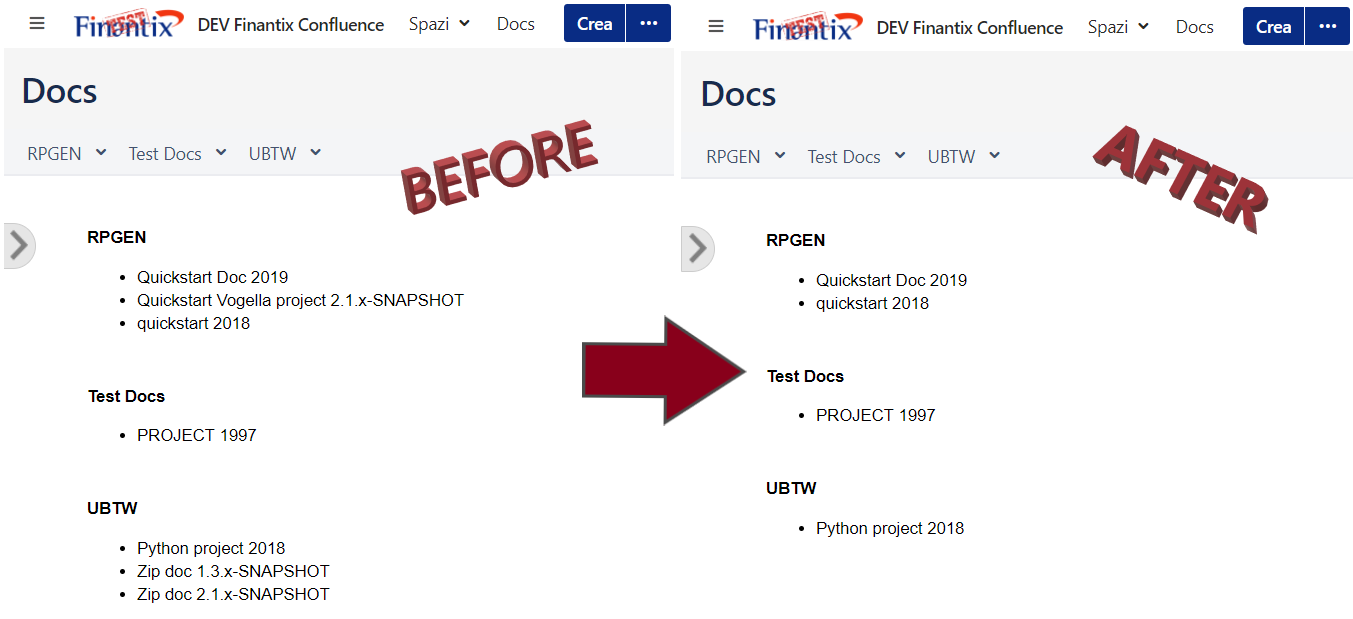
\includegraphics[width=\textwidth]{cleanup3D}\\
	\caption{Esempio di Docs prima e dopo l'esecuzione del goal \emph{cleanup}}
	\label{cleanupBeforeAfter}
\end{figure}



% Furthermore a doc page can be overall identified by its docKey, which is a sequence of category id and doc id.


\section{Raccolta dei requisiti}
Il momento dell'analisi e raccolta dei requisiti è avvenuto in congiunzione con il tutor aziendale.
In principio è stato discusso dei prodotti principali da realizzare, quali plugin e documentazione. 
Dopodiché si è proseguiti con il dettaglio delle loro caratteristiche, come per esempio gli artefatti compresi nella documentazione e i precisi compiti del plugin.
Tutti i requisiti identificati sono stati riportati in specifici ticket in Jira, lo strumento di monitoraggio delle attività di riferimento per tutti gli sviluppatori dell'azienda.
Ogni ticket possiede un identificativo univoco e specifica un compito da svolgere; citiamo per esempio:
\begin{itemize}
	\item creazione di un ``hello world'' (prototipo semplice) plugin Maven;
	\item implementazione del plugin Maven per la pubblicazione di documentazione;
	\item creazione manuale dello sviluppatore;
	\item creazione manuale per l'utente.
\end{itemize}
Ognuno di questi ticket ha un proprio flusso di lavoro predefinito o personalizzabile in base alla modalità di lavoro \cite{site:jira}.
In questo caso, essendo il progetto portato avanti da una persona singola sequenzialmente, il flusso comprendeva gli stati di base:
\begin{enumerate}
	\item \bd{TO DO}: attività da svolgere;
	\item \bd{IN PROGRESS}: attività iniziata da completare;
	\item \bd{DONE}: attività completata.
\end{enumerate} 
% Lo stato veniva gradualmente aggiornato dalla candidata.
Ogni ticket viene associato ad una pagina di Confluence, appositamente creata in parallelo, che possiede una struttura ben delineata.
Essa spiega nel modo più specifico possibile il ticket a cui è collegato: quale necessità ne ha spinta la creazione, che cosa ne consegue, ecc.
Viene innanzitutto riportata la \emph{user story}, ovvero la descrizione del linguaggio naturale e informale di una o più funzionalità di un sistema software \cite{site:user-story}, comprendente le informazioni riguardanti a: la persona che richiede che l'attività venga svolta, qual è esattamente il compito e per quale motivo deve essere svolto.
Per esempio, nel caso della pagina Confluence legata al ticket della creazione del manuale utente, questa era: \\
\emph{As a developer \\
I want a guide for the Maven documentation publisher plug-in \\
so that can easily configure it for my Java project.} \\
Successivamente alla user story, nella pagina Confluence  gli artefatti tecnici, ovvero il dettaglio delle caratteristiche del ticket.
Nel caso dell'implementazione del plugin Maven, questi erano:
\begin{itemize}
	\item informazioni sulla repository di Bitbucket in cui deve risiedere il codice sorgente;
	\item informazioni sull'identificazione del plugin;
	\item configurazione desiderata;
	\item comportamento desiderato;
	\item scenari di test;
	\item goal extra;
	\item configurazioni extra.
\end{itemize}


\clearpage

\section{Requisiti}	\label{requisiti}
Ad ogni requisito viene assegnato il codice identificativo univoco:
	\begin{center}
		\texttt{R[Numero][Tipo][Priorità]}
	\end{center}
	in cui ogni parte ha un significato preciso:
	\begin{itemize}
		\item \textbf{R}: requisito.
		\item \textbf{Numero}: numero progressivo che segue una struttura gerarchica.
		\item \textbf{Tipo}: la la tipologia di requisito che può essere di:
		\begin{itemize}
			\item \textbf{F}: funzionalità.
			\item \textbf{Q}: qualità.
			\item \textbf{V}: vincolo.
		\end{itemize}
		\item \textbf{Priorità}: indica il grado di urgenza di un requisito di essere soddisfatto, come:
		\begin{itemize}
			\item \textbf{0}: opzionale.
			\item \textbf{1}: desiderabile.
			\item \textbf{2}: obbligatorio.
		\end{itemize}
	\end{itemize}

	Esempio: \texttt{R2Q1} indica il secondo requisito di qualità ed è desiderabile. \\

	I requisiti individuati sono riassunti in tabelle secondo la loro tipologia.
	Inoltre, tutti i requisiti individuati e scelti dalla candidata, presentano nella tabella come fonte ``Interno'' e come grado di urgenza ``0'' poiché il loro soddisfacimento non è richiesto.


% Da un'attenta analisi dei requisiti e dei casi d'uso effettuata sul progetto, è stata stilata la tabella che traccia tutti i requisiti in rapporto alle loro fonti.

% \newpage


	\subsection{Requisiti di funzionalità} \label{requisitiFunzionalita}
	I requisiti di funzionalità sono ulteriormente suddivisi in tabelle secondo:
	\begin{itemize}
		\item requisiti relativi a ciò che il sistema permette all'utente di configurare;
		\item requisiti relativi a messaggi di errore che il sistema deve essere in grado di lanciare;
		\item requisiti relativi a generiche funzionalità del sistema.
	\end{itemize}
	Per ogni tabella, i primi requisiti, segnalati come obbligatori, sono i requisiti identificati all'inizio del progetto, essenziali per il funzionamento del plugin.
	I requisiti elencati successivamente come desiderabili sono invece le funzionalità aggiunte in un secondo momento, nel corso dello stage, come quanto accennato nella premessa all'inizio di questo capitolo.
	All'interno della descrizione del requisito si utilizzano alcune abbreviazioni per semplificare la lettura della tabella:
	\begin{itemize}
		\item ``Inserimento'' per ``L'utente nella configurazione deve poter inserire'';
		\item ``Errore se'' per ``Il sistema deve dare un messaggio di errore qualora''.
	\end{itemize}
		 

	% \stepcounter{tableCounter}
	\begin{table}[H]
		\begin{paddedtablex}[1.7]{\textwidth}{cXc}%0 opz  2 obb
			\rowcolor{beautyblue} \textbf{Codice} & \textbf{Descrizione} & \textbf{Fonte} \\\toprule
			
			\ReqF{2}{Inserimento documentazione}{Azienda}
				\subReqF{2}{Inserimento archivio (ZIP o JAR)}{Azienda}
				\subReqF{1}{Inserimento file HTML}{Azienda}
				\subReqF{1}{Inserimento cartella}{Azienda}	
            \ReqF{2}{Inserimento credenziali}{Azienda}
			    \subReqF{2}{Inserimento username}{Azienda}
				\subReqF{2}{Inserimento password}{Azienda}
				\subReqF{2}{Inserimento identificativo server}{Azienda}
			\ReqF{2}{Inserimento nome della categoria Confluence in cui allocare la documentazione}{Azienda}	
			\ReqF{2}{Inserimento nome della documentazione}{Azienda}
			\ReqF{2}{Inserimento versione della documentazione}{Azienda}
			\ReqF{2}{L'utente deve poter configurare il plugin in modo che esso ne salti la propria esecuzione}{Azienda}
			\ReqF{1}{Inserimento luogo in cui l'archivio viene salvato all'interno del progetto}{Azienda}
			\ReqF{1}{Inserimento tipologie di file attinenti alla documentazione}{Azienda}
				\ReqF{1}{Inserimento tipologie di file da includere nell'archivio}{Azienda}
				\ReqF{1}{Inserimento tipologie di file da escludere dall'archivio}{Azienda}
			\ReqF{1}{Inserimento nome del file principale della documentazione}{Azienda}
			\ReqF{1}{L'utente deve poter configurare il plugin in modo che esso non fallisca se avvengono errori del client}{Azienda}
			\ReqF{1}{Inserimento tipi di progetto supportati dal plugin}{Azienda}
			\ReqF{1}{Inserimento tipi di progetto a cui il plugin non deve dare messaggi di warning}{Azienda}
			\ReqF{1}{L'utente deve poter configurare il plugin in modo che esso non fallisca se l'archivio dato non esiste}{Azienda}
			
			\bottomrule
		\end{paddedtablex}
		\caption{Elenco dei requisiti di funzionalità relativi alla configurazione}
	\end{table}


	\begin{table}[H]
		\begin{paddedtablex}[1.7]{\textwidth}{cXc}%0 opz  2 obb
			\rowcolor{beautyblue} \textbf{Codice} & \textbf{Descrizione} & \textbf{Fonte} \\\toprule
			
			\ReqF{2}{Errore se l'utente non fornisce nessuna documentazione}{Azienda}
			\ReqF{2}{Errore se l'archivio dato non esiste}{Azienda}	
			\ReqF{2}{Errore se l'utente non fornisce le proprie credenziali}{Azienda}
			\ReqF{2}{Errore se l'utente non fornisce il nome della categoria}{Azienda}
			\ReqF{1}{Errore se il file indicato dall'utente, come file principale della cartella, non esiste}{Azienda}

			\bottomrule
		\end{paddedtablex}
		\caption{Elenco dei requisiti di funzionalità relativi ai messaggi di errore
		% (\thetableCounter)
		}
	\end{table}

	\begin{table}[H]
		\begin{paddedtablex}[1.7]{\textwidth}{cXc}%0 opz  2 obb
			\rowcolor{beautyblue} \textbf{Codice} & \textbf{Descrizione} & \textbf{Fonte} \\\toprule

			\ReqF{2}{Il sistema deve fornire delle proprietà per tutti gli elementi configurabili dall'utente}{Azienda}
			\ReqF{2}{Il sistema deve essere in grado di costruire il titolo della pagina contenente la documentazione, a partire da nome e versione della documentazione}{Azienda}
			\ReqF{1}{Il sistema deve permettere lo skip dell'esecuzione del plugin, nel caso in cui il progetto compilato non sia tra i tipi supportati}{Azienda}
			\ReqF{1}{L'utente deve poter eliminare tutta la documentazione con versione ``SNAPSHOT'' presente}{Azienda}

			\bottomrule
		\end{paddedtablex}
		\caption{Elenco dei requisiti di funzionalità del sistema
		% (\thetableCounter)
		}
	\end{table}



	% \setcounter{tableCounter}{1}
	% NB: molti requisiti di qualità sono stati tolti perchè non sono veri requisiti del sistema, riguardano noi e il nostro modo di fare, non il sistema
	\subsection{Requisiti di qualità}\label{RequisitiQualita}


	\begin{table}[H]
		\begin{paddedtablex}[1.7]{\textwidth}{cXc}
			\rowcolor{beautyblue}\textbf{Codice} & \textbf{Descrizione} & \textbf{Fonte} \\
			\toprule
			
			\ReqQ{2}{Le norme presenti sulla wiki aziendale devono essere rispettate}{Azienda}
				% \subReqQ{1}{Ogni commit effettuato deve rispettare la formattazione descritta nella wiki}{Azienda}
				\subReqQ{2}{Il nome di ogni variabile, classe e metodo nel codice deve essere significativo}{Azienda}
				\subReqQ{2}{I commenti nel codice devono essere facilmente comprensibili}{Azienda}
				\subReqQ{2}{Il codice non deve contenere violazioni di SonarQube con alta severità}{Azienda}
				\subReqQ{2}{La copertura dei test deve essere almeno pari al 70\% del codice}{Azienda}

			\bottomrule
		\end{paddedtablex}
		\caption{Elenco dei requisiti di qualità (1)}
	\end{table}


	\begin{table}[H]
		\begin{paddedtablex}[1.7]{\textwidth}{cXc}
			\rowcolor{beautyblue}\textbf{Codice} & \textbf{Descrizione} & \textbf{Fonte} \\
			\toprule

			\ReqQ{2}{Devono essere forniti test realizzati con JUnit che verifichino la copertura di tutti i parametri disponibili nella configurazione}{Azienda}
			\ReqQ{2}{Deve essere redatto un manuale utente}{Azienda}
				\subReqQ{2}{Deve essere redatta una pagina Confluence che descriva come configurare il plugin}{Azienda}
				\subReqQ{1}{Deve essere redatta una pagina di utilizzo Maven ``Usage'' che descriva tutti i possibili utilizzi del plugin}{Azienda}
			\ReqQ{2}{Deve essere redatto un manuale sviluppatore}{Azienda}
				\subReqQ{2}{Deve essere redatta una pagina Confluence che descriva la progettazione del plugin tramite diagrammi}{Azienda}
				\subReqQ{2}{Deve essere redatta e generata la documentazione Javadoc del plugin}{Azienda}
			\ReqQ{0}{Il nome di ogni test realizzato con JUnit deve iniziare con ``test''}{Interno}
			\ReqQ{0}{Il nome di ogni test realizzato con JUnit deve rispettare la notazione camel case}{Interno}
			\ReqQ{0}{Ogni messaggio di errore del plugin deve essere sufficientemente esplicativo}{Interno}

			\bottomrule
		\end{paddedtablex}
		\caption{Elenco dei requisiti di qualità (2)}
	\end{table}



	\subsection{Requisiti di vincolo}\label{RequisitiVincolo}

	\begin{table}[H]
		\begin{paddedtablex}[1.7]{\textwidth}{cXc}
			\rowcolor{beautyblue}\textbf{Codice} & \textbf{Descrizione} & \textbf{Fonte} \\
			\toprule

			\ReqV{2}{Il plugin deve essere sviluppato nel linguaggio di programmazione Java}{Azienda}
			\ReqV{2}{Il plugin deve essere testato tramite JUnit}{Azienda}
			\ReqV{2}{Come ambiente di sviluppo è necessario utilizzare Eclipse}{Azienda}
			\ReqV{2}{Per la build dei progetti è necessario utilizzare Maven}{Azienda}
			\ReqV{2}{Per la pubblicazione di documentazione è necessario utilizzare Confluence}{Azienda}


			\bottomrule
		\end{paddedtablex}
		\caption{Elenco dei requisiti di vincolo (1)}
	\end{table}


	\begin{table}[H]
		% \centering
		% {\def\arraystretch{1.7}
		% \begin{tabularx}{\textwidth}{cXc}
		\begin{paddedtablex}[1.7]{\textwidth}{cXc}
			\rowcolor{beautyblue}\textbf{Codice} & \textbf{Descrizione} & \textbf{Fonte} \\
			\toprule

			\ReqV{2}{I requisiti identificati devono essere tracciati su Jira}{Azienda}
			\subReqV{2}{Lo stato di ogni requisito presente su Jira deve sempre essere opportunamente aggiornato}{Azienda}
			\ReqV{2}{Come strumento di continuous integration è necessario utilizzare Jenkins}{Azienda}
			\ReqV{2}{Per l'analisi statica del codice è necessario utilizzare SonarQube}{Azienda}
			\ReqV{2}{Per il controllo di versione del codice è necessario utilizzare Bitbucket}{Azienda}
			\ReqV{2}{Utilizzare JUnit per realizzare test di unità}{Azienda}
			\ReqV{0}{Utilizzare GitKraken come client di Git}{Interno}
			\ReqV{0}{Utilizzare Visual Studio Code come editor per il codice}{Interno}
			\ReqV{0}{Utilizzare SequenceDiagram.org per la creazione dei diagrammi di sequenza}{Interno}
			\ReqV{0}{Utilizzare ObjectAid UML Explorer per la creazione dei diagrammi delle classi}{Interno}
			\ReqV{0}{Utilizzare Meecrowave per la creazione di un semplice server}{Interno}

			\bottomrule
		\end{paddedtablex}
		\caption{Elenco dei requisiti di vincolo (2)}
	\end{table}


	\subsection{Riepilogo dei requisiti}

	\begin{table}[H]
		\centering
		{\def\arraystretch{1.7}
		\begin{tabularx}{\textwidth}{XXXX}
			\rowcolor{beautyblue} \textbf{Tipologia} & \textbf{Obbligatori} & \textbf{Desiderabili} & \textbf{Opzionali} \\\toprule
			Di funzionalità & 16 & 14 & 0 \\
			Di qualità & 11 & 1 & 3 \\
			Di vincolo & 11 & 0 & 5
			\\\bottomrule
		\end{tabularx}}
		\caption{Riepilogo dei requisiti}
	\end{table}


	\section{Tracciamento dei requisiti}

	\begin{table}[H]
		{\def\arraystretch{1.5}
		\begin{tabularx}{\textwidth}{XX}
			\rowcolor{beautyblue}
			\textbf{Codice} &
			\textbf{Fonte} \\ \hline
			R1F2 & Azienda \\
			R1.1F2 & Azienda \\
			R1.2F1 & Azienda \\
			R1.3F1 & Azienda \\
			R2F2 & Azienda \\
			R2.1F2 & Azienda \\
			R2.2F2 & Azienda \\
			R2.3F2 & Azienda \\
			R3F2 & Azienda \\
			R4F2 & Azienda \\
			R5F2 & Azienda \\
			R6F2 & Azienda \\
			R7F1 & Azienda \\
			R8F1 & Azienda \\
			R9F1 & Azienda \\
			R10F1 & Azienda \\
			R11F1 & Azienda \\
			R12F1 & Azienda \\
			R13F1 & Azienda \\
			R14F1 & Azienda \\
			R15F1 & Azienda \\
			R16F2 & Azienda \\
			R17F2 & Azienda \\
			R18F2 & Azienda \\
			R19F2 & Azienda \\
			R20F1 & Azienda \\
			R21F2 & Azienda \\

			\bottomrule
		\end{tabularx}} 
	\caption{Requisiti in rapporto alle fonte ``Azienda'' (1)}
	\end{table}

	\begin{table}[H]
		{\def\arraystretch{1.5}
		\begin{tabularx}{\textwidth}{XX}
			\rowcolor{beautyblue}
			\textbf{Codice} &
			\textbf{Fonte} \\ \hline
			
			R22F2 & Azienda \\
			R23F1 & Azienda \\
			R24F1 & Azienda \\
			R1Q2 & Azienda \\
			R1.1Q2 & Azienda \\
			R1.2Q2 & Azienda \\
			R1.3Q2 & Azienda \\
			R1.4Q2 & Azienda \\
			R2Q2 & Azienda \\
			R3Q2 & Azienda \\
			R3.1Q2 & Azienda \\
			R3.2Q1 & Azienda \\
			R4Q2 & Azienda \\
			R4.1Q2 & Azienda \\
			R4.2Q2 & Azienda \\
			R1V2 & Azienda \\
			R2V2 & Azienda \\
			R3V2 & Azienda \\
			R4V2 & Azienda \\
			R5V2 & Azienda \\
			R6V2 & Azienda \\
			R6.1V2 & Azienda \\
			R7V2 & Azienda \\
			R8V2 & Azienda \\
			R9V2 & Azienda \\
			R10V2 & Azienda \\

			\bottomrule
		\end{tabularx}} \\
	\caption{Requisiti in rapporto alla fonte ``Azienda'' (2)}
	\end{table}


	\begin{table}[H]
		{\def\arraystretch{1.5}
		\begin{tabularx}{\textwidth}{XX}
			\rowcolor{beautyblue}
			\textbf{Codice} &
			\textbf{Fonte} \\ \hline
			R5Q0 & Interno \\
			R6Q0 & Interno \\
			R7Q0 & Interno \\
			R11V0 & Interno \\
			R12V0 & Interno \\
			R13V0 & Interno \\
			R14V0 & Interno \\
			R15V0 & Interno \\
			%  & Interno \\
			%  & Interno \\
			%  & Interno \\
			%  &  \\
			%  &  \\
			%  &  \\
			%  &  \\
		\end{tabularx}} \\
	\caption{Requisiti in rapporto alla fonte ``Interno''}
	\end{table}






% \begin{table}%
% \caption{Tabella del tracciamento dei requisiti di vincolo}
% \label{tab:requisiti-vincolo}
% \begin{tabularx}{\textwidth}{lXl}
% \hline\hline
% \textbf{Requisito} & \textbf{Descrizione} & \textbf{Use Case}\\
% \hline
% RVO-1    & La libreria per l'esecuzione dei test automatici deve essere riutilizzabile & - \\
% \hline
% \end{tabularx}
% \end{table}%             % Concept Preview
% !TEX encoding = UTF-8
% !TEX TS-program = pdflatex
% !TEX root = ../tesi.tex

%**************************************************************
\chapter{Progettazione} %TODO e codifica
\label{cap:progettazione}
%**************************************************************

\intro{Breve introduzione al capitolo}\\

%**************************************************************
\section{Tecnologie e strumenti} %TODO vedere se serve
\label{sec:tecnologie-strumenti}

Di seguito viene data una panoramica delle tecnologie e strumenti utilizzati.

\subsection*{Tecnologia 1}
Descrizione Tecnologia 1.

\subsection*{Tecnologia 2}
Descrizione Tecnologia 2

%**************************************************************
\section{Ciclo di vita del software}
\label{sec:ciclo-vita-software}

%**************************************************************
\section{Progettazione}
\label{sec:progettazione}

% \subsubsection{Namespace 1} %**************************
% Descrizione namespace 1.

% \begin{namespacedesc}
%     \classdesc{Classe 1}{Descrizione classe 1}
%     \classdesc{Classe 2}{Descrizione classe 2}
% \end{namespacedesc}


%**************************************************************
\section{Design Pattern utilizzati}

%**************************************************************
% \section{Codifica}
             % Product Prototype
% !TEX encoding = UTF-8
% !TEX TS-program = pdflatex
% !TEX root = ../tesi.tex

%**************************************************************
\chapter{Verifica e validazione}
\label{cap:testing} % TODO sistemare riferimenti

\section{Analisi statica}
L'analisi statica relizzata grazie all'utilizzo di SonarQube.
La sua esecuzione veniva messa in atto ogni qual volta avveniva una build di Jenkins.
I problemi che SonarQube può segnalare, possono essere di tre tipi:
\begin{itemize}
    \item \bd{bug}: un errore nel codice che richiede di essere corretto il prima immediatamente;
    \item \bd{vulnerabilità}: un punto nel codice che è aperto agli attacchi;
    \item \bd{codesmell}:  un problema di manutenibiltià che rende il codice confuso e difficile da manutenere.
\end{itemize}
Ognuno dei quali può avere un grado di severità differente, ordinate dalla più alla meno importante:
\begin{itemize}
    \item \bd{BLOCKER}
    \item \bd{CRITICAL}
    \item \bd{MAJOR}
    \item \bd{MINOR}
    \item \bd{INFO}.
\end{itemize}

La maggior parte dei problemi segnalati da SonarQube durante il progetto, erano codesmell di diversa severità MINOR o MAJOR.
Per il termine del progetto, la totalità di quelli etichettati come MAJOR sono stati risolti, come richiesto dalle norme aziendali relative al codice, ma anche molti dei MINOR.
 


\section{Test di unità}

L'attività di testing per quel che riguarda i test di unità è stata svolta utilizzando principalmente due framework: JUnit e Mockito.

    \subsection{JUnit}


    \subsection{Mockito}



\section{Test di validazione}


%**************************************************************             % Product Design Freeze e SOP
% !TEX encoding = UTF-8
% !TEX TS-program = pdflatex
% !TEX root = ../tesi.tex

%**************************************************************
\chapter{Conclusioni}
\label{cap:conclusioni}
%**************************************************************

%**************************************************************
\section{Risultato ottenuto}
% uguale a intro ma con riferimenti più specifici a quanto già detto
....

%**************************************************************
\section{Analisi critica del prodotto e del lavoro di stage}
......


%**************************************************************
\subsection{Utilizzazione del prodotto} %Il prodotto è utilizzato?
Maven documentation publisher plug-in non è ancora stato messo in produzione ma diventerà a breve il metodo ufficiale di pubblicazione della documentazione sul sistema aziendale Confluence.


%**************************************************************
\subsection{Valutazione degli strumenti utilizzati}
......

%**************************************************************
\subsection{Possibili punti di insoddisfazione}
......

\subsubsection{Relativi miglioramenti}
......

%**************************************************************
\subsection{Possibili estensioni}
......             % Conclusioni
\appendix
% !TEX encoding = UTF-8
% !TEX TS-program = pdflatex
% !TEX root = ../tesi.tex

%**************************************************************
% \chapter{Glossario}
% %**************************************************************

% % \epigraph{Citazione}{Autore della citazione}
% \section*{A}
%     \subsection*{API REST}
%     Le ..

% % \section*{B}
% %     \subsection*{B-word}
% %     Ecc..

% % \section*{C}    


% \section*{J}
%     \subsection*{Jenkins}
%     ....

%     \subsection*{Jira}
%     .....
             % Appendice A

%**************************************************************
% Materiale finale
%**************************************************************
\backmatter
\printglossaries
% !TEX encoding = UTF-8
% !TEX TS-program = pdflatex
% !TEX root = ../tesi.tex

%**************************************************************
% Bibliografia
%**************************************************************

\cleardoublepage
\chapter{Bibliografia}

\nocite{*}
% Stampa i riferimenti bibliografici
% \printbibliography[heading=subbibliography,title={Riferimenti bibliografici},type=book]

% Stampa i siti web consultati
\printbibliography[heading=subbibliography,title={Siti web consultati},type=online]


% @book{womak:lean-thinking,
%     author  = {James P. Womack, Daniel T. Jones},
%     title   = {Lean Thinking, Second Editon},
%     publisher = {Simon \& Schuster, Inc.},
%     year    = {2010}
% }
\end{document}
